\documentclass{article}

\usepackage{amsmath}
\usepackage{amsfonts} % For math fonts.
\usepackage{amssymb} % For other math symbols not covered by amsmath.
\usepackage[pdftex]{graphicx} % For pictures, use \includegraphics[scale=decimal]{pic.png}; must be a .png file type.
\usepackage{multicol}
\usepackage{textcomp}
\usepackage[colorlinks = true, urlcolor = blue]{hyperref}
\usepackage{enumitem}
\usepackage{graphbox} 
\usepackage{subfig}
\usepackage{multicol}
\usepackage{nopageno}
\usepackage{bm}


\usepackage{tikz}
\usetikzlibrary{positioning, calc}
\usetikzlibrary{shapes.geometric,angles,quotes}
\usepackage{tikz-3dplot}


%page formatting
\usepackage{fullpage}
\setlength{\parindent}{0pt}


\newcommand{\tab}{\hspace*{0.25in}}
\newcommand{\csq}[1]{\reflectbox{''}#1''}  %This produces CS style quotes.
\newcommand{\csqt}[1]{\text{\reflectbox{''}#1''}}  %This produces CS style quotes as text.


\usepackage{listings}
\lstset
{ %Formatting for code in appendix
    language=Python,
    basicstyle=\footnotesize,
    numbers=left,
    stepnumber=1,
    showstringspaces=false,
    tabsize=2,
    breaklines=true,
    breakatwhitespace=false,
}


\begin{document}



%split_point

%\end{document}
Lone Star \hfill midterm retake quiz\\
section 4\\
\begin{enumerate}
\item (8.2)
	Write a \textbf{function} that takes a list of \textbf{ingredients} and returns the total 
	\textbf{cost} of making a recipe. You may use the following dictionary named $prices$:
	\begin{center}
		prices = \{ \csq{flour} : 2.50, \csq{sugar} : 1.80, \csq{eggs} : 3.00, \csq{milk} : 2.00, 
			\csq{butter} : 2.75, \csq{vanilla} : 4.50, \csq{chocolate} : 5.00 \}
	\end{center}
	Hint: You can calculate the total cost by summing up the prices of all valid ingredients in 
	the list.  You may assume the \textit{prices} dictionary is defined in your code.  You don't 
	need to rewrite it.
	
	\textbf{Examples:}  
	\begin{itemize}  
		\item total\_cost([\csq{flour}, \csq{sugar}, \csq{eggs}, \csq{butter}]) $\rightarrow$ 10.05
		\item total\_cost([\csq{milk}, \csq{vanilla}, \csq{chocolate}]) $\rightarrow$ 11.50
		\item total\_cost([\csq{eggs}, \csq{eggs}, \csq{flour}, \csq{sugar}]) $\rightarrow$ 10.30
	\end{itemize}



\item (6.1)
		Write a function called \textit{flip\_flop} that takes a string as an argument 
		and returns  a new word made up of the second half of the word first combined 
		with the first half of the word second.

		\textbf{Examples:}
		\begin{itemize}
			\item \textit{flip\_flop}(\csq{abcd}) $\rightarrow$ \csq{cdab} 
				(that is, \csq{cd} then \csq{ab} \dots even length)
			\item \textit{flip\_flop}(\csq{grapes}) $\rightarrow$ \csq{pesgra} 
				(that is, \csq{pes} then \csq{gra} \dots even length)
			\item \textit{flip\_flop}(\csq{abcde})$\rightarrow$ \csq{decab}
				(that is, \csq{de} then \csq{c} then \csq{ab} \dots odd length)
			\item \textit{flip\_flop}(\csq{cranberries})$\rightarrow$ \csq{rriesecranb}
				(that is, \csq{rries} then \csq{e} then \csq{cranb} \dots odd length)

		\end{itemize}

%end_of_questions



\item (8.3)
	Write a \textbf{function} that takes a dictionary, called $store$, representing items and their prices, and an integer, called $wallet$, 
	representing the amount of money you have. The function should return a list of items you can afford.
	If you cannot afford anything, return an empty list.

	\textbf{Examples:}  
	\begin{itemize}  
		\item items\_purchase(\{\csq{Water}: 1, \csq{Bread}: 3, \csq{TV}: 1000\}, 300) $\rightarrow$ [\csq{Bread}, \csq{Water}]
		\item items\_purchase(\{\csq{Apple}: 4, \csq{Pan}: 100, \csq{Spoon}: 2 \}, 100) $\rightarrow$ [\csq{Apple}, \csq{Pan}, \csq{Spoon}]
		\item items\_purchase(\{\csq{Phone}: 999, \csq{Laptop}: 5000, \csq{PC}: 1200 \}, 1) $\rightarrow$ []
	\end{itemize}  



\end{enumerate}
\pagebreak
Dot Matrix \hfill midterm retake quiz\\
section 5\\
\begin{enumerate}
\item (4.1)  
		Write a program that asks the user for a word and then, \underline{using a loop}, 
		prints every other letter of the word starting with the second letter.

		Examples:
		\begin{itemize}
			\item if user\_word = \csq{counterattack}, the result should be \csq{oneatc}
			\item if user\_word = \csq{banana sunday}, the result should be \csq{aaasna}
		\end{itemize}


\item (3.1)  
		Write a program that prompts the user for a letter and checks whether the letter is a vowel 
		or consonant.  A vowel should output \textit{\csq{vowel}}, and a consonant should output 
		\textit{consonant}.  You may assume only lower case letters. Below is sample output.\\
		Hint: In the English language, a, e, i, o, and u are the vowels.
	
		\begin{figure}[h]
		\centering
			\begin{minipage}{.5\textwidth}
			\centering
				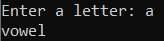
\includegraphics[scale=1.2]{./imgs/vowelYesAlt.png}
			\end{minipage}%
				%
			\begin{minipage}{.5\textwidth}
			\centering
				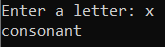
\includegraphics[scale=1.1]{./imgs/vowelNoAlt.png}
			\end{minipage}
		\end{figure}





\item (3.2)  
		Write a program that prompts the user to enter three integers and displays the integers 
		in decreasing order (largest to smallest).  You may not use the built-in functions 
		\textit{max}(), \textit{min}(), \textit{sort}() or \textit{sorted}().



\end{enumerate}
\pagebreak
Dark Helmet \hfill midterm retake quiz\\
section 4\\
\begin{enumerate}
\item (4.2)  
		%https://edabit.com/challenge/ksZrMdraPqHjvbaE6
		Write a program that repeatedly asks the user for integers until a negative integer is 
		given.\\  Report back the largest \textbf{even} number the user entered 
		(not including the negative number).  \\
		If the user didn't enter any even numbers report back $-1$.

		For example, \\ \ \hfill
		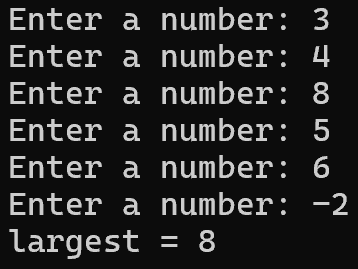
\includegraphics[height = 1.2in]{./imgs/largestEven1.PNG} \hfill  
		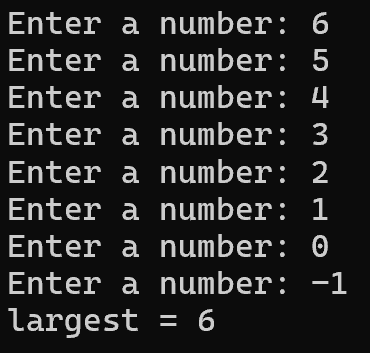
\includegraphics[height = 1.5in]{./imgs/largestEven2.PNG} \hfill  
		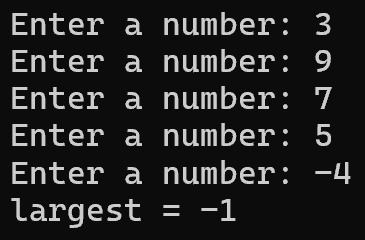
\includegraphics[height = 1.2in]{./imgs/largestEven3.PNG} \hfill \

%end_of_questions

\item (2.1)
		%https://edabit.com/challenge/QzXtDnSZL6y4ZcEvT
		A farmer is asking you to tell him how many legs can be counted among all his animals. 
		The farmer breeds three species:
		\begin{itemize}
			\item chickens, which have \textbf{2} legs
			\item cows, which have \textbf{4} legs
			\item pigs, which have \textbf{4} legs
		\end{itemize}
		Write a program that asks the farmer how many of each animal he has, and then outputs the
		total number of legs.  		
		For example, \\ \ \hfill
		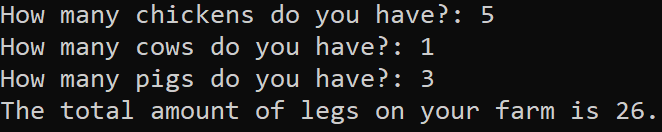
\includegraphics[height = 0.6in]{./imgs/animalLegs_ex1.PNG} \hfill
		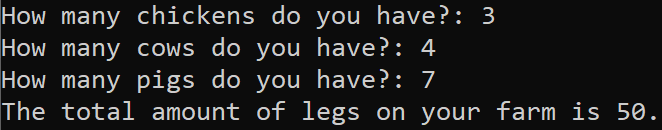
\includegraphics[height = 0.6in]{./imgs/animalLegs_ex2.PNG} \hfill \



\end{enumerate}
\pagebreak
President Skroob \hfill midterm retake quiz\\
section 1\\
\begin{enumerate}
\item (2.1)
		%https://edabit.com/challenge/QzXtDnSZL6y4ZcEvT
		A farmer is asking you to tell him how many legs can be counted among all his animals. 
		The farmer breeds three species:
		\begin{itemize}
			\item chickens, which have \textbf{2} legs
			\item cows, which have \textbf{4} legs
			\item pigs, which have \textbf{4} legs
		\end{itemize}
		Write a program that asks the farmer how many of each animal he has, and then outputs the
		total number of legs.  		
		For example, \\ \ \hfill
		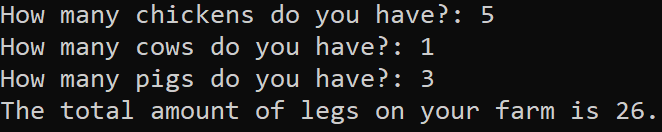
\includegraphics[height = 0.6in]{./imgs/animalLegs_ex1.PNG} \hfill
		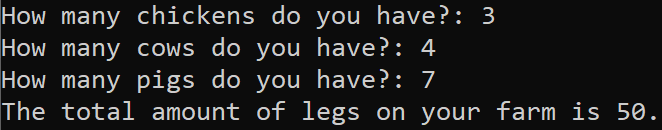
\includegraphics[height = 0.6in]{./imgs/animalLegs_ex2.PNG} \hfill \


\item (4.2)  
		%https://edabit.com/challenge/ksZrMdraPqHjvbaE6
		Write a program that repeatedly asks the user for integers until a negative integer is 
		given.\\  Report back the largest \textbf{even} number the user entered 
		(not including the negative number).  \\
		If the user didn't enter any even numbers report back $-1$.

		For example, \\ \ \hfill
		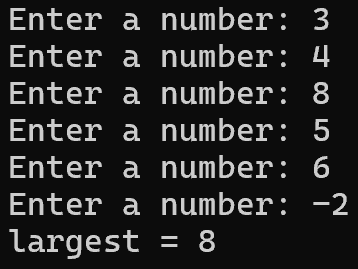
\includegraphics[height = 1.2in]{./imgs/largestEven1.PNG} \hfill  
		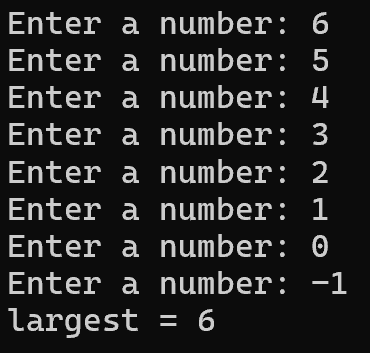
\includegraphics[height = 1.5in]{./imgs/largestEven2.PNG} \hfill  
		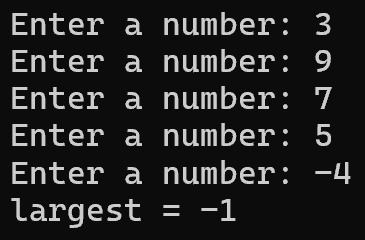
\includegraphics[height = 1.2in]{./imgs/largestEven3.PNG} \hfill \

%end_of_questions

\item (3.3)  
		The table below shows what time different age groups (by grade) can swim at the pool.  There 
		are two time options, morning and afternoon.  Write a program that asks the user their grade 
		and whether they'd like to go in the morning or afternoon, and outputs the time the pool is 
		available for them.

		\begin{minipage}{.45\textwidth}
		\begin{tabular}{c|cc}
						& \multicolumn{2}{c}{Pool times}\\
			Grade 		& Morning 	& Afternoon \\ \hline
			k, 1 -- 3 	& 9 AM 		& 1 PM\\
			4 -- 8 		& 10 AM 	& 2 PM\\
			9 -- 12 	& 11 AM 	& 3 PM \\
		\end{tabular}
		\end{minipage}
		%
		\begin{minipage}{.45\textwidth}
			\ \\
			Your end output should look similar to this
			%(if you were to actually run the code).

			\fbox{\parbox{\textwidth}{ Enter your grade: 5\\
			Enter Morning OR Afternoon: Morning\\
			The pool is open at 10 AM.}}
		\end{minipage}



%end_of_questions








\item (1.2) Write a program that asks the user for \\
		\begin{minipage}{0.5\textwidth}
		\vspace*{-0.5em}
			\begin{enumerate}  \setlength\itemsep{-0.3em}
				\item their first name and
				\item their age.  
			\end{enumerate} \vspace*{-1ex}
		and then outputs a greeting.
		\end{minipage}
		%\
		\begin{minipage}{0.5\textwidth}
			\centering
			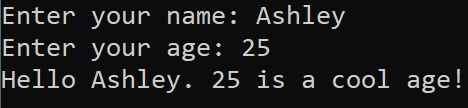
\includegraphics[scale=0.95]{./imgs/outputGreetingWithAge.png}\\
			Your output should be similar to this.
		\end{minipage}




\item (3.1)  
		%https://edabit.com/challenge/8pDH2SRutPoaQghgc
		Luke Skywalker has friends and family, but he is getting older and having trouble 
		remembering them all.  Write a program that Luke (the user) can input a name and it 
		outputs the relation defined in the table below.
		\begin{center}
		\begin{tabular}{|l|l|} \hline
			Person 		& Relation \\ \hline \hline
			Darth Vader	& Father \\ \hline
			Leia		& Sister \\ \hline
			Han			& Brother in law\\ \hline
			R2D2		& Droid \\ \hline
		\end{tabular}\\ \hspace*{1in} *If he types any other name, report \csq{unknown}.
		\end{center}
		


%end_of_questions





\end{enumerate}
\pagebreak
\end{document}